\chapter{Projekt systemu (Piotr Chojnowski)}
\label{chap:project}

Projekt ma za cel stworzenie aplikacji wirtualnego escape roomu do nauki fizyki dla szkoły średniej. Poniższy rozdział przedstawia organizacyjne i projektowe założenia stojące za realizacją aplikacji.

\section{Zespół i harmonogram prac}
Zespół projektowy składa się z czterech studentów:

\begin{itemize} 
    \item Michał Kortas -- Kierownik zespołu z doświadczeniem w modelowaniu 3D w środowisku Blender. Posiada również podstawowe doświadczenie z zakresu projektowania gier komputerowych oraz obsługi silnika Unreal Engine.
    \newline
    \item Piotr Chojnowski -- Posiada podstawowe doświadczenie w programowaniu gier komputerowych oraz obsłudze silnika Unreal Engine. Dodatkowo ma umiejętności w tworzeniu tekstur.
    \newline
    \item Kamil Danecki -- Członek koła naukowego VERTEX zajmującego się tworzeniem gier komputerowych. Doświadczenie w projektowaniu gier oraz obsłudze silnika Unreal Engine.
    \newline
    \item Paweł Januszczak -- Posiada podstawowe doświadczenie w projektowaniu gier komputerowych oraz obsłudze silnika Unreal Engine. Znajomość programowania dla środowiska VR.
\end{itemize}
\hfill
\newline
\begin{table}
    \centering
    \begin{tabular}{ |p{3cm}|p{8cm}|  }
     \hline
     \textbf{Miesiąc} & \textbf{Zadania} \\ 
     \hline
     Luty & Ustalenie ogólnych wymagań. \\
     \hline
     Marzec & Analiza narzędzi i dotychczasowych rozwiązań. \newline 
     Projekt pierwszych zagadek. \\   
     \hline
     Kwiecień & Konsultacje z ekspertem. \newline 
     Projekt pozostałych zagadek. \newline
     Stworzenie mechanizmów poruszania się oraz interakcji z otoczeniem.\\ 
     \hline
     Maj & Implementacja zagadek z mechaniki, termodynamiki oraz drgań. \newline
     Wytworzenie potrzebnych modeli 3D do tych zagadek. \\
     \hline
     Czerwiec & Testy w środowisku CAVE. \newline
     Implementacja zagadek z fizyki atomowej oraz prądu elektrycznego. \newline 
     Wytworzenie potrzebnych modeli 3D do tych zagadek. \\  
     \hline
     Lipiec & Implementacja zagadek z fal i optyki oraz elementów fizyki relatywistycznej i fizyki jądrowej. \newline 
     Wytworzenie potrzebnych modeli 3D do tych zagadek. \\ 
     \hline
     Sierpień & Implementacja zagadek z grawitacji i elementów astronomii oraz mechaniki bryły sztywnej. \newline 
     Wytworzenie potrzebnych modeli 3D do tych zagadek. \\ 
     \hline
     Wrzesień & Implementacja zagadek z elektrostatyki oraz magnetyzmu \newline 
     Wytworzenie potrzebnych modeli 3D do tych zagadek. \\ 
     \hline
     Październik & Testy w środowisku CAVE. \newline
     Poprawy w zagadkach. \\ 
     \hline
     Listopad & Poprawki graficzne. \newline
     Testy przeprowadzone przez osoby trzecie. \\ 
     \hline
     Grudzień & Dokończenie dokumentacji. \\
     \hline
    \end{tabular}
    \caption{Harmonogram pracy}
    \label{tab:harmonogram}
\end{table}
    
\section{Specyfikacja wymagań}
Aplikacja ma być grą zespołową w stylu escape room na system CAVE. Ma zawierać co najmniej 11 zagadek - po jednej zagadce z każdej dziedziny fizyki na poziomie szkoły średniej: mechanika, mechanika bryły sztywnej, grawitacja i elementy astronomii, drgania, termodynamika, elektrostatyka, prąd elektryczny, magnetyzm, fale i optyka, fizyka atomowa, elementy fizyki relatywistycznej i fizyka jądrowa.

\section{Ogólna struktura aplikacji}
Aplikacja ma postać 12 pokoi w rozmiarze 3.4m x 3.4m x 3.4m. Pierwszy pokój pełni funkcję menu głównego i wstępu, a każdy pozostały pokój zawiera rozbudowaną zagadkę z jednej z 11 dziedzin fizyki na poziomie szkoły średniej.

\begin{figure}[h!]
    \centering
    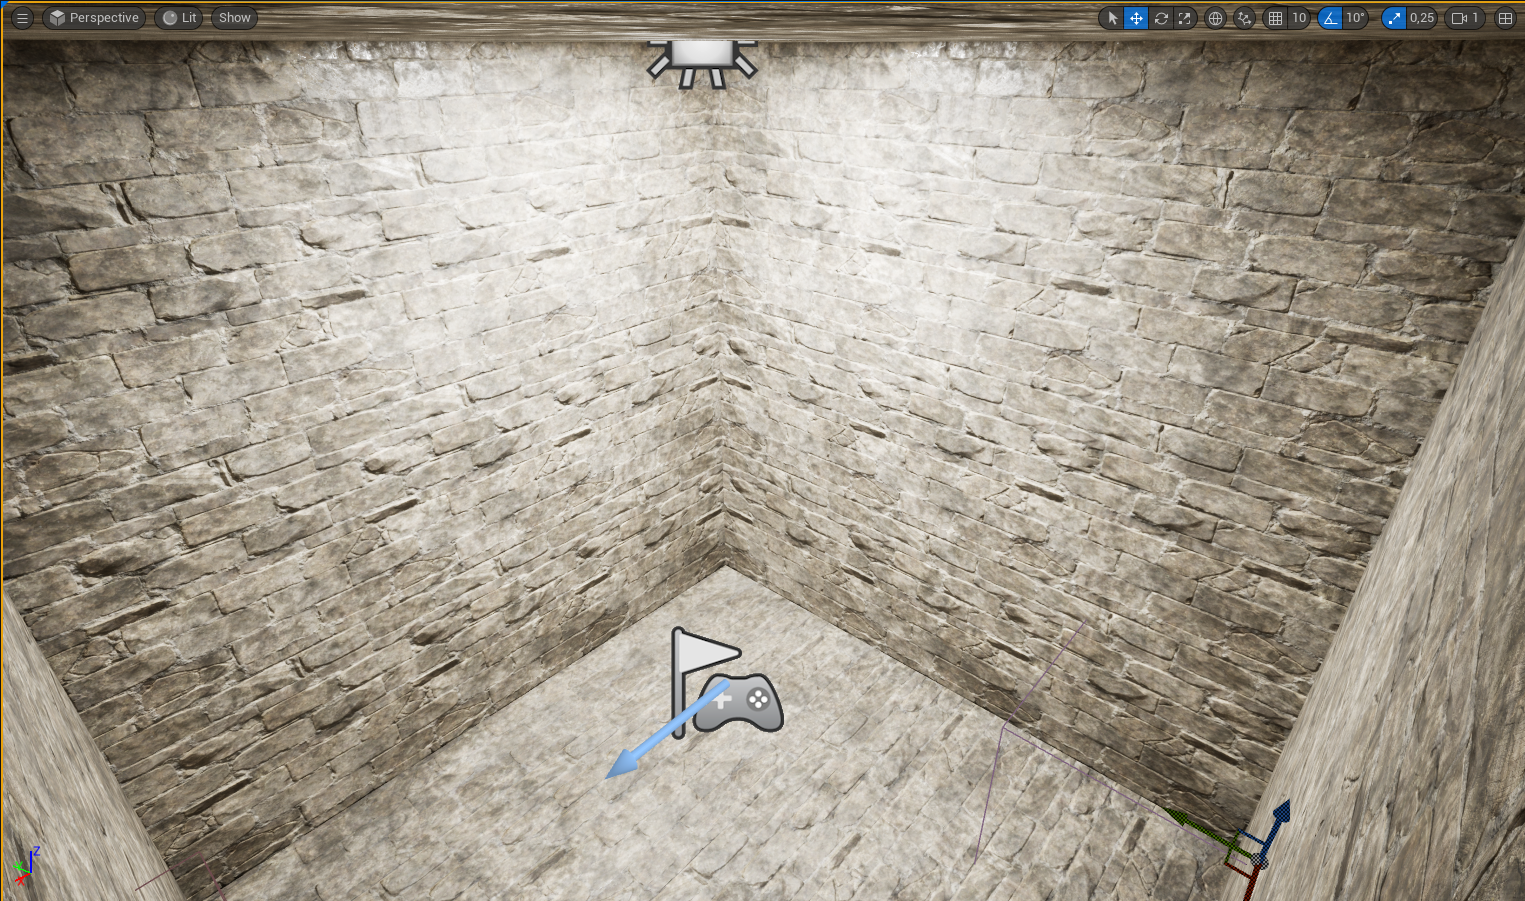
\includegraphics[width=0.6\textwidth]{images/empty_room.png}
    \caption{Przykład pustego pokoju przed implementacją zagadki}
    \label{img:empty_room}
\end{figure}

Gracz zaczyna w pierwszym pokoju. Po rozwiązaniu w nim zagadki przechodzi do kolejnego, wygrywa, gdy ukończy ostatni pokój.\

\section{Projekty zagadek}

Program składa się z 11 różnych zagadek. Zostały one opisane poniżej.

\subsection{Zagadka z mechaniki}
W ramach zagadki z mechaniki gracz będzie musiał użyć drewnianych belek, aby zbudować most, który wytrzyma ciężar przejeżdżającego po nim pojazdu. Na środku pokoju znajduje się miniaturowy wąwóz. Gracz ma limitowaną ilość belek. Gdy pojazd przejedzie na drugą stronę wąwozu, zagadka jest zaliczona jako ukończona.

\subsection{Zagadka z mechaniki bryły sztywnej}
Na środku pokoju znajduje się tarcza zegara ze wskazówką sekund. Zegar jest zatrzymany. Gracz musi właściwie rozmieścić ciężarki, aby zegar zaczął chodzić z odpowiednią prędkością.

\subsection{Zagadka z grawitacji i elementów astronomii}
Aby rozwiązać zagadkę, gracz musi odpowiednio ustawić miniaturowe ciała niebieskie w odpowiednim dystansie i z odpowiednią prędkością, aby ustabilizować układ. Zagadka liczy się jako ukończona, jeżeli układ był stabilny przez ciąg 5-ciu sekund.

\subsection{Zagadka z drgań}
Gracz musi nastroić odpowiednio harfę, aby jej struny wydawały dźwięk o odpowiedniej częstotliwości, a następnie zagrać je w odpowiedniej kolejności, aby odtworzyć melodię składającą się z 5-ciu nut. Zagadka liczy się jako ukończona po zagraniu pełnej melodii.

\subsection{Zagadka z termodynamiki}
Gracz wciela się w kowala, który musi odpowiednio utrzymać temperaturę sztabki żelaza, aby była wystarczająco plastyczna, by uderzając młotem uformować ją w broń. Zagadka liczy się jako zaliczona, gdy broń zostanie uformowana.

\subsection{Zagadka z elektrostatyki}
Zagadka z elektrostatyki stawia gracza w różnych polach elektrostatycznych, gdzie gracz musi dobrać ładunki tak, aby ustabilizować ruch cząsteczek w tych polach. Zagadka liczy się jako ukończona po ustabilizowaniu 3 pól ze zwiększającym się poziomem skomplikowania.

\subsection{Zagadka z prądu elektrycznego}
Zagadka z prądu elektrycznego polega na uzupełnieniu układu elektrycznego, aby dostarczał wystarczające napięcie prądu, jednocześnie nie spalając układu. Gracz dostosowuje parametry elementów, takich jak rezystory, zasilanie i połączenia przewodników. Zagadka liczy się jako ukończona, gdy gracz ukończy dwa układy - pierwszy służy jako poradnik wyjaśniający sterowanie.

\subsection{Zagadka z magneryzmu}
W pokoju znajdują się różnego kształtu magnesy. Gracz musi odpowiednio ustawić linie pól magnetycznych, aby odpowiadały rzeczywistości. Zagadka liczy się jako zaliczona, gdy wszystkie pola są poprawne.

\subsection{Zagadka z fali i optyki}
Zagadka z fali i optyki polega na odpowiednim ustawieniu poprawnych soczewek w lukach w labiryncie na ścianie, tak aby wiązka światła dotarła do jego końca. Przy drugiej ścianie znajduje się stół z różnymi opisanymi soczewkami, które gracz może wybrać. Gracz używa kontrolera, aby przenosić soczewki, które automatycznie wchodzą do luki, gdy są wystarczająco blisko niej. Zagadka liczy się jako ukończona, gdy wiązka światła przejdzie przez labirynt.

\subsection{Zagadka z fizyki atomowej}
Gracz wchodzi w skalę mikro i odpowiednio przesuwa elektrony po orbitach, aby utworzyć z atomów izotopy, a następnie połączyć je w związek. Zagadka liczy się jako ukończona po utworzeniu związku.

\subsection{Zagadka z elementów fizyki relatywistycznej i fizyki jądrowej}
W pokoju znajdują się różne radioaktywne elementy z opisami. Gracz musi odpowiednio je posortować rosnąco zgodnie z ich czasem rozkładu połowicznego. Zagadka liczy się jako zakończona, gdy wszystkie elementy są na ich odpowiednim miejscu. 

